\documentclass[a4paper,11pt]{report}
\usepackage{chuan_math_gkt}
\usetikzlibrary{angles,quotes,intersections,patterns,decorations.pathreplacing}
\chuanexamsetup

\begin{document}
\examfontsize

\examsecret{绝密$\bigstar$启用前}

\examtitle{2023年普通高等学校招生全国统一考试（全国乙卷理科）}{数\quad 学}

\noticetitle
\begin{examnotice}
\item 答卷前，考生务必将自己的姓名、准考证号填写在答题卡上. 
\item 回答选择题时，选出每小题的答案后，用铅笔把答题卡上对应题目的答案标号涂黑. 如需改动，用橡皮擦干净后，再选涂其他答案标号. 回答非选择题时，将答案写在答题卡上. 写在本试卷上无效. 
\item 考试结束后，将本试卷和答题卡一并交回. 
\end{examnotice}

\examsection{一、选择题：本题共12小题，每小题5分，共60分. 在每小题给出的四个选项中，只有一项是符合题目要求的. }
\begin{examquestions}
\item 设$z=\dfrac{2+\mathrm{i}}{1+\mathrm{i}^2+\mathrm{i}^5}$，则$\overline z=$
\fourchoices{$1-2\mathrm{i}$}{$1+2\mathrm{i}$}{$2-\mathrm{i}$}{$2+\mathrm{i}$}
\item 设集合$U=\mathbb R$，集合$M=\{x\mid x<1\}$，$N=\{x\mid -1<x<2\}$，则$\{x\mid x\geq2\}=$
\twochoices{$\complement_U(M\cup N)$}{$N\cup\complement_U M$}{$\complement_U(M\cap N)$}{$M\cup\complement_U N$}
\item 如图，网格纸上绘制的一个零件的三视图，网格小正方形的边长为$1$，则该零件的表面积为
\begin{tightcenter}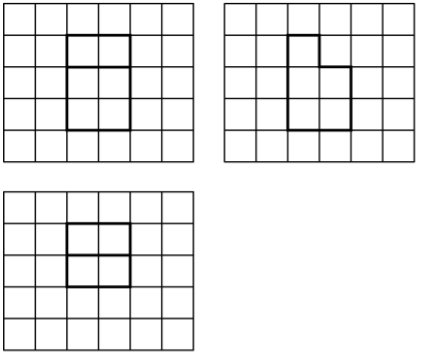
\includegraphics[width=2.7cm]{figures/2023_yi_li_q3.png}\end{tightcenter}
\fourchoices{$24$}{$26$}{$28$}{$30$}
\item 已知$f(x)=\dfrac{xe^x}{e^{ax}-1}$是偶函数，则$a=$
\fourchoices{$-2$}{$-1$}{$1$}{$2$}
\item 设$O$为平面坐标系的坐标原点，在区域$\{(x,y)\mid 1\leq x^2+y^2\leq4\}$内随机取一点，记该点为$A$，则直线$OA$的倾斜角不大于$\dfrac\pi4$的概率为
\fourchoices{\tallchoice{$\dfrac18$}}{\tallchoice{$\dfrac16$}}{\tallchoice{$\dfrac14$}}{\tallchoice{$\dfrac12$}}
\item 已知函数$f(x)=\sin(\omega x+\varphi)$在区间$\left(\dfrac\pi6,\dfrac{2\pi}3\right)$单调递增，直线$x=\dfrac\pi6$和$x=\dfrac{2\pi}3$为函数$y=f(x)$的图像的两条对称轴，则$f\left(-\dfrac{5\pi}{12}\right)=$
\fourchoices{\tallchoice{$-\dfrac{\sqrt3}{2}$}}{\tallchoice{$-\dfrac12$}}{\tallchoice{$\dfrac12$}}{\tallchoice{$\dfrac{\sqrt3}{2}$}}
\item 甲乙两位同学从$6$种课外读物中各自选读$2$种，则这两人选读的课外读物中恰有$1$种相同的选法共有
\fourchoices{$30$种}{$60$种}{$120$种}{$240$种}
\item 已知圆锥$PO$的底面半径为$\sqrt3$，$O$为底面圆心，$PA,PB$为圆锥的母线，$\angle AOB=120^\circ$，若$\triangle PAB$的面积等于$\dfrac{9\sqrt3}{4}$，则该圆锥的体积为
\fourchoices{$\pi$}{$\sqrt6\pi$}{$3\pi$}{$3\sqrt6\pi$}
\item 已知$\triangle ABC$为等腰直角三角形，$AB$为斜边，$\triangle ABD$为等边三角形，若二面角$C-AB-D$为$150^\circ$，则直线$CD$与平面$ABC$所成角的正切值为
\fourchoices{\tallchoice{$\dfrac15$}}{\tallchoice{$\dfrac{\sqrt2}{5}$}}{\tallchoice{$\dfrac{\sqrt3}{5}$}}{\tallchoice{$\dfrac25$}}
\item 已知等差数列$\{a_n\}$的公差为$\dfrac{2\pi}3$，集合$S=\{\cos a_n\mid n\in\mathbb N^*\}$，若$S=\{a,b\}$，则$ab=$
\fourchoices{$-1$}{\tallchoice{$-\dfrac12$}}{$0$}{\tallchoice{$\dfrac12$}}
\item 设$A,B$为双曲线$x^2-\dfrac{y^2}{9}=1$上两点，下列四个点中，可为线段$AB$中点的是
\fourchoices{$(1,1)$}{$(-1,2)$}{$(1,3)$}{$(-1,-4)$}
\item 已知$\odot O$的半径为$1$，直线$PA$与$\odot O$相切于点$A$，直线$PB$与$\odot O$交于$B,C$两点，$D$为$BC$的中点，若$|PO|=\sqrt2$，则$\vec{PA}\cdot\vec{PD}$的最大值为
\fourchoices{\tallchoice{$\dfrac{1+\sqrt2}{2}$}}{\tallchoice{$\dfrac{1+2\sqrt2}{2}$}}{$1+\sqrt2$}{$2+\sqrt2$}
\end{examquestions}

\examsection{二、填空题：本题共4小题，每小题5分，共20分. }
\begin{examquestions}[start=13]
\item 已知点$A(1,\sqrt5)$在抛物线$C:y^2=2px$上，则$A$到$C$的准线的距离为\blank. 
\item 若$x,y$满足约束条件\linsys{x-3y\leq -1,\\x+2y\leq9,\\3x+y\geq7}，则$z=2x-y$的最大值为\blank. 
\item 已知$\{a_n\}$为等比数列，$a_2a_4a_5=a_3a_6$，$a_9a_{10}=-8$，则$a_7=$\blank. 
\item 设$a\in(0,1)$，若函数$f(x)=a^x+(1+a)^x$在$(0,+\infty)$上单调递增，则$a$取值范围是\blank. 
\end{examquestions}

\examsection{三、解答题：本题共6小题，共70分. 解答应写出文字说明、证明过程或演算步骤. }
\begin{examanswers}[start=17]
\item（12分）

某厂为比较甲乙两种工艺对橡胶产品伸缩率处理效应，进行$10$次配对试验，每次配对试验选用材质相同的两个橡胶产品，随机地选其中一个用甲工艺处理，另一个用乙工艺处理，测量处理后的橡胶产品的伸缩率，甲、乙两种工艺处理后的橡胶产品的伸缩率分别记为$x_i,y_i(i=1,2,\cdots,10)$，试验结果如下：
\begin{tightcenter}
{\renewcommand{\arraystretch}{0.9}
\begin{tabular}{|c|*{10}{c|}}
\hline 试验序号$i$ & 1&2&3&4&5&6&7&8&9&10\\\hline
伸缩率$x_i$ & 545&533&551&522&575&544&541&568&596&548\\\hline
伸缩率$y_i$ & 536&527&543&530&560&533&522&550&576&536\\\hline
\end{tabular}}
\end{tightcenter}
记$z_i=x_i-y_i(i=1,2,\cdots,10)$，记$z_1,z_2,\ldots,z_{10}$的样本平均数为$\bar z$，样本方差为$s^2$. 

\subq{（1）}{求$\bar z$，$s^2$；}

\subq{（2）}{判断甲工艺处理后的橡胶产品的伸缩率较乙工艺处理后的橡胶产品的伸缩率是否有显著提高（如果$\bar z\geq2\sqrt{\dfrac{s^2}{10}}$，则认为有显著提高，否则不认为有显著提高）.}

\item（12分）

在$\triangle ABC$中，已知$\angle BAC=120^\circ$，$AB=2$，$AC=1$. 

\subq{（1）}{求$\sin\angle ABC$；}

\subq{（2）}{若$D$为$BC$上一点，且$\angle BAD=90^\circ$，求$\triangle ADC$的面积.}

\item（12分）

如图，在三棱锥$P-ABC$中，$AB\perp BC$，$AB=2$，$BC=2\sqrt2$，$PB=PC=\sqrt6$，$BP,AP,BC$的中点分别为$D,E,O$，$AD=\sqrt5DO$，点$F$在$AC$上，$BF\perp AO$. 

\noindent\begin{minipage}[t]{0.64\linewidth}
\subq{（1）}{证明：$EF\parallel$平面$ADO$；}

\subq{（2）}{证明：平面$ADO\perp$平面$BEF$；}

\subq{（3）}{求二面角$D-AO-C$的正弦值.}
\end{minipage}\hfill
\begin{minipage}[t]{0.34\linewidth}
\vspace{-1.5em}
\centering
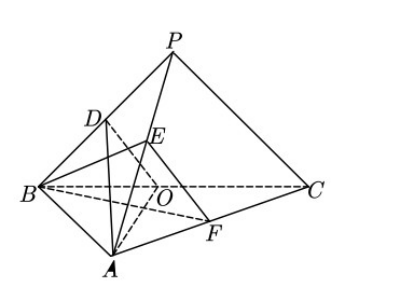
\includegraphics[width=\linewidth]{figures/2023_yi_li_q19.png}
\end{minipage}
\vspace{-3em}
\item（12分）

已知椭圆$C:\dfrac{y^2}{a^2}+\dfrac{x^2}{b^2}=1(a>b>0)$的离心率为$\dfrac{\sqrt5}{3}$，点$A(-2,0)$在$C$上. 

\subq{（1）}{求$C$的方程；}

\subq{（2）}{过点$(-2,3)$的直线交$C$于点$P,Q$两点，直线$AP,AQ$与$y$轴的交点分别为$M,N$，证明：线段$MN$的中点为定点.}

\item（12分）

已知函数$f(x)=\left(\dfrac1x+a\right)\ln(1+x)$. 

\subq{（1）}{当$a=-1$时，求曲线$y=f(x)$在点$(1,f(1))$处的切线方程；}

\subq{（2）}{是否存在$a,b$，使得曲线$y=f\left(\dfrac1x\right)$关于直线$x=b$对称，若存在，求$a,b$的值，若不存在，说明理由；}

\subq{（3）}{若$f(x)$在$(0,+\infty)$存在极值，求$a$的取值范围.}
\end{examanswers}

\vspace{1em}
\begin{examanswers}[start=22]
\item（10分）【选修4-4：坐标系与参数方程】

在直角坐标系$xOy$中，以坐标原点$O$为极点，$x$轴正半轴为极轴建立极坐标系，曲线$C_1$的极坐标方程为$\rho=2\sin\theta\left(\dfrac\pi4\leq\theta\leq\dfrac\pi2\right)$，曲线$C_2:$\linsys{x=2\cos\alpha,\\y=2\sin\alpha}（$\alpha$为参数，$\dfrac\pi2<\alpha<\pi$）. 

\subq{（1）}{写出$C_1$的直角坐标方程；}

\subq{（2）}{若直线$y=x+m$既与$C_1$没有公共点，也与$C_2$没有公共点，求$m$的取值范围.}

\item（10分）【选修4-5：不等式选讲】

已知$f(x)=2|x|+|x-2|$. 

\subq{（1）}{求不等式$f(x)\leq6-x$的解集；}

\subq{（2）}{在直角坐标系$xOy$中，求不等式组\linsys{f(x)\leq y,\\x+y-6\leq0}所确定的平面区域的面积.}
\end{examanswers}

\end{document}
